\documentclass{beamer}

\mode<presentation>
{
	\usetheme{CambridgeUS}
	\setbeamercovered{transparent}
}

\usepackage[spanish]{babel}
\usepackage[latin1]{inputenc}
\usepackage{color}
\usepackage{hyperref}
\usepackage{algorithm,algorithmic}
\usepackage{colortbl}
\usepackage{graphicx}

\title[\textbf{Programaci\'on 2}]{\textbf{Programaci\'on 2}}

\subtitle{Lenguaje Java - Conceptos claves}

%\author[Rodrigo Olivares]
%{
%	Rodrigo Olivares \\
%	\vspace{0.5mm}
%	Mg. en Ingenier\'ia Inform\'atica \\
%	\vspace{0.5mm}
%	\texttt{\normalsize rodrigo.olivares@uv.cl}
%}
\author[Eduardo Godoy]
{
	Profesor: Eduardo Godoy \\
	\vspace{0.5mm}
	\texttt{\normalsize eduardo.gl@gmail.coml} \\ 
	Material elaborado por Rodrigo Olivares \\
	\texttt{\normalsize rodrigo.olivares@uv.cl} 
}

\institute[Universidad de Valpara\'iso]

%\date{$2^{do}$ Semestre de 2016}

%\subject{Programaci\'on 2}
%
%\AtBeginSection
%{
%	\begin{frame}<beamer>
%	\frametitle{Contenido}
%	\tableofcontents[currentsection,currentsubsection]
%	\end{frame}
%}
%
%\AtBeginSubsection
%{
%	\begin{frame}<beamer>
%	\frametitle{Contenido}
%	\tableofcontents[currentsection,currentsubsection]
%	\end{frame}
%}
%
%\beamerdefaultoverlayspecification{<+->}

\begin{document}

	\begin{frame}
		\titlepage
	\end{frame}

	\begin{frame}
		\frametitle{Contenido}
		\tableofcontents%[pausesections]
	\end{frame}

    \section{Comportamiento principal}
    
		\subsection{Constructor}

        \begin{frame}
			\frametitle{Comportamiento Principal}
			\framesubtitle{Constructor}

			\begin{block}{}
			    \begin{itemize}
                    \item[-] En programaci\'on orientada a objetos (POO), un \textbf{constructor} es una m\'etodo cuya misi\'on es inicializar un objeto de una clase. En el constructor se asignan los valores iniciales del nuevo objeto.
                    \item[-] Debe tener el \textbf{mismo nombre de la Clase}.
                    \item[-] En Java, el constructor es un m\'etodo \emph{especial} dentro de una clase, que se llama autom\'aticamente cada vez que se instancia un objeto de esa clase.
                    \item[-] Una clase puede no tener un constructor. En este caso, el compilador de Java crea uno vac\'io.
                    \item[-] Una clase puede tener m\'as de un constructor. \'Estos se diferencian por los par\'ametros que recibe (\emph{sobrecarga de m\'etodo}).
                \end{itemize}
			\end{block}
		\end{frame}

        \begin{frame}
			\frametitle{Comportamiento Principal}
			\framesubtitle{Bloques}

			\begin{block}{}
				    \begin{itemize}
                    				\item Inicializaci\'on: Se ejecutan cuando una una clase es instanciada. Incluso antes del constructor.
 					\item Est\'aticos: A diferencia de los de Inicializaci\'on, se ejecutan cuando una una clase es cargada.
				\end{itemize}
			\end{block}
		\end{frame}


        \begin{frame}
			\frametitle{Comportamiento Principal}
			\framesubtitle{Constructor}

			\begin{block}{}
				{\scriptsize
				\textcolor{blue}{public class} \textbf{\emph{Auto}} \{ \\
				\hspace{1cm} \\
				\hspace{1cm} \textcolor{blue}{private} String \textcolor{green}{color}; \ \\
				\hspace{1cm} \textcolor{blue}{private} String \textcolor{green}{marca}; \ \\
				\hspace{1cm} \textcolor{blue}{private} \textcolor{blue}{boolean} \textcolor{green}{estado}; \ \\
				\hspace{1cm} \\
				\hspace{1cm} \textcolor{blue}{public} \textbf{Auto}() \{ \\
				\hspace{1cm} \} \\
				\hspace{1cm} \\
				\hspace{1cm} \textcolor{blue}{public} \textbf{Auto}(String color) \{ \\
				\hspace{2cm} \textcolor{blue}{this}.\textcolor{green}{color} = color; \\
				\hspace{1cm} \} \\
				\hspace{1cm} \\
				\hspace{1cm} \textcolor{blue}{public} \textbf{Auto}(String color, String marca) \{ \\
				\hspace{2cm} \textcolor{blue}{this}.\textcolor{green}{color} = color; \\
				\hspace{2cm} \textcolor{blue}{this}.\textcolor{green}{marca} = marca; \\
				\hspace{1cm} \} \\
				\}}
			\end{block}
		\end{frame}

    \section{Lectura de datos}
    
		\subsection{BufferedReader/InputStreamReader}
		
		\begin{frame}
			\frametitle{Lectura de datos}
			\framesubtitle{BufferedReader/InputStreamReader}

            \begin{block}{Nos apoyamos en la clase System}
				{\scriptsize
				\textcolor{blue}{public class} \textbf{\emph{AutoImpl}} \{ \\
				\hspace{1cm} \\
				\hspace{1cm} \textcolor{blue}{public static void} \textbf{main}(String[ ] args) \{ \\
				\hspace{2cm} String texto; \\
				\hspace{2cm} BufferedReader br = \textcolor{blue}{new} BufferedReader(\textcolor{blue}{new} InputStreamReader(System.\textcolor{green}{\emph{in}})); \\
				\hspace{2cm} \textcolor{blue}{do} \{ \\
				\hspace{3cm} System.\emph{\textcolor{green}{out}}.println(\textcolor{orange}{''Ingreso algun texto''});\\
				\hspace{3cm} texto = br.\emph{readLine}();\\
				\hspace{3cm} System.\emph{\textcolor{green}{out}}.println(texto);\\
				\hspace{2cm} \} \textcolor{blue}{while}(!sTexto.\emph{equals}(\textcolor{orange}{''FIN''})); \\
				\hspace{1cm} \} \\
				\}}
			\end{block}
		\end{frame}		
		
		\subsection{Scanner}

        \begin{frame}
			\frametitle{Lectura de datos}
			\framesubtitle{Scanner}

            \begin{block}{Nos apoyamos en la clase System}
				{\scriptsize
				\textcolor{blue}{public class} \textbf{\emph{AutoImpl}} \{ \\
				\hspace{1cm} \\
				\hspace{1cm} \textcolor{blue}{public static void} \textbf{main}(String[ ] args) \{ \\
				\hspace{2cm} String texto; \\
				\hspace{2cm} Scanner s = \textcolor{blue}{new} Scanner(System.\textcolor{green}{\emph{in}});\\
				\hspace{2cm} \textcolor{blue}{do} \{ \\
				\hspace{3cm} System.\emph{\textcolor{green}{out}}.println(\textcolor{orange}{''Ingreso algun texto''});\\
				\hspace{3cm} texto = s.\emph{nextLine}();\\
				\hspace{3cm} System.\emph{\textcolor{green}{out}}.println(texto);\\
				\hspace{2cm} \} \textcolor{blue}{while}(!sTexto.\emph{equals}(\textcolor{orange}{''FIN''})); \\
				\hspace{1cm} \} \\
				\}}
			\end{block}
		\end{frame}	

        \begin{frame}
			\frametitle{Lectura de datos}
			\framesubtitle{Scanner}

            \begin{block}{Algunos m\'etodos de la clase Scanner}
				{\scriptsize
				    \begin{itemize}
                        \item[-] \emph{nextBoolean}(): Scans the next token of the input into a boolean value and returns that value.
                        \item[-] \emph{nextByte}(): Scans the next token of the input as a byte.
                        \item[-] \emph{nextDouble}(): Scans the next token of the input as a double.
                        \item[-] \emph{nextFloat}(): Scans the next token of the input as a float.
                        \item[-] \emph{nextInt}(): Scans the next token of the input as an int.
                        \item[-] \emph{nextLine}(): Advances this scanner past the current line and returns the input that was skipped.
                        \item[-] \emph{nextLong}(): Scans the next token of the input as a long.
                        \item[-] \emph{nextShort}(): Scans the next token of the input as a short.
                        \item[ ] ...
                        \item[ ] Revisar API \emph{http://docs.oracle.com/javase/6/docs/api/}
                    \end{itemize}
				}
			\end{block}
		\end{frame}	

    \section{Argumentos principales}
    
		\subsection{Lectura de argumentos}
		
		\begin{frame}
			\frametitle{Argumentos Principales}
			\framesubtitle{Lectura de argumentos}

			\begin{block}{}
			    {\scriptsize
                    \textquestiondown C\'omo podemos leer una lista de argumentos ingresados al momento de ejecutar el c\'odigo?
			    }
			\end{block}
			\begin{block}{}
				{\scriptsize
				\textcolor{blue}{public class} \textbf{\emph{AutoImpl}} \{ \\
				\hspace{1cm} \\
				\hspace{1cm} \textcolor{blue}{public static void} \textbf{main}(String[ ] args) \{ \\
				\hspace{2cm} \textcolor{blue}{for}(\textcolor{blue}{int} i = 0: i $<$ args.length; i++) \{ \\
				\hspace{3cm} System.\emph{\textcolor{green}{out}}.println(args[i]);\\
				\hspace{2cm} \} \\
				\hspace{1cm} \} \\
				\}}
			\end{block}
			\begin{block}{}
			    {\scriptsize
                    \$ \emph{java} Auto Chevrolet Camaro amarillo 24000000
			    }
			\end{block}
		\end{frame}

	\section{Almacenamiento m\'ultiple}

		\subsection{Arreglos}

		\begin{frame}
			\frametitle{Almacenamiento M\'ultiples}
			\framesubtitle{Arreglos}

			\begin{block}{}
			    {\scriptsize
				Los arreglos son una forma de almacenar una lista de elementos. Cada espacio/celda del arreglo guarda un elemento individual. Los arreglos pueden tener cualquier tipo de dato (primitivos u objetos), pero \textbf{no puede almacenar distintos tipos en un mismo arreglo}.
			    }
			\end{block}
			\begin{block}{}
			    {\scriptsize
				    Para crear un arreglo se debe: 
                    \begin{itemize}
                        \item Declarar una variable para guardar el arreglo.
                        \item Crear/instanciar un nuevo objeto de arreglo y asignarlo a la variable de arreglo.
                        \item Almacenar los valores en el arreglo.
                    \end{itemize}
			    }
			\end{block}
		\end{frame}

		\begin{frame}
			\frametitle{Almacenamiento M\'ultiples}
			\framesubtitle{Arreglos}

			\begin{block}{Declaraci\'on}
			    {\scriptsize
				    Las variables de arreglo indican el tipo de objeto que el arreglo contendr\'a y el nombre del arreglo. Los corchetes vac\'ios pueden incluirse despu\'es del tipo de dato o despu\'es del nombre del arreglo, indistintamente.
			    }
			\end{block}
			\begin{block}{}
			    {\scriptsize
                \begin{itemize}
                    \item[] \textbf{String} \emph{palabras[]};
                    \item[] \textbf{int} \emph{vertices[]};
                    \item[] \textbf{Personas} \emph{personas[]};
                    \item[] \textbf{String[]} \emph{palabras};
                    \item[] \textbf{int[]} \emph{vertices};
                    \item[] \textbf{Personas[]} \emph{personas};
                 \end{itemize}
			    }
			\end{block}
		\end{frame}

        \begin{frame}
			\frametitle{Almacenamiento M\'ultiples}
			\framesubtitle{Arreglos}

			\begin{block}{Instanciaci\'on}
			    {\scriptsize
				    Usar \textbf{new}:
				    \begin{itemize}
                        \item[] Por ejemplo, \textbf{String[]} \emph{nombre} = \textbf{new String[}\emph{10}\textbf{]};
                    \end{itemize}
                    Esta linea crea un arreglo de String con 10 espacios/celdas. \textbf{Siempre} que se instancie un arreglo con \textbf{new} se debe indicar de que tama\~no ser\'a (n\'umero de celdas).
			    }
			\end{block}
			\begin{block}{}
			    {\scriptsize
			    El arreglo se inicializar\'a con : 
                \begin{itemize}
                    \item $0$ para arreglos num\'ericos.
                    \item \textbf{false} para booleanos.
                    \item $'/0'$  para arreglos de caracter.
                    \item \textbf{null} para objetos.
                 \end{itemize}
			    }
			\end{block}
		\end{frame}

        \begin{frame}
			\frametitle{Almacenamiento M\'ultiples}
			\framesubtitle{Arreglos}

			\begin{block}{Instanciaci\'on}
			    {\scriptsize
				    Por extensi\'on:
				    \begin{itemize}
                        \item[] Por ejemplo, \textbf{String[]} \emph{nombre = \{''pedro'', ''rodrigo'', ''carlo'', ''andres''\}};
                    \end{itemize}
			    }
			\end{block}
			\begin{block}{Instanciaci\'on}
			    {\scriptsize
				    Cada elemento dentro de las llaves debe ser del mismo tipo y coincidir con el tipo de variable que contiene el arreglo
			    }
			\end{block}
		\end{frame}
   
        \begin{frame}
			\frametitle{Almacenamiento M\'ultiples}
			\framesubtitle{Arreglos}

			\begin{block}{Acceso al dato}
			    {\scriptsize
				    Para acceder a un elemento del arreglo se usan los sub-\'indices:
				    \begin{itemize}
                        \item[] \textbf{String[]} texto = \textbf{new String[}10\textbf{]};
                        \item[] \emph{texto}[9] = ''test'';
                        \item[] \textbf{int} largoTexto = texto.\emph{length};
                     \end{itemize}
			    }
			\end{block}
			\begin{block}{}
			    {\scriptsize
                     La \'ultima l\'inea de c\'odigo permite ver la longitud del arreglo. Este atributo est\'a disponible para todos los objetos arreglo sin importar el tipo. En java no es posible asignar un valor, a una celda fuera del l\'imite de \'este. Los subindices se inician en 0.
			    }
			\end{block}
		\end{frame}

        \begin{frame}
			\frametitle{Almacenamiento M\'ultiples}
			\framesubtitle{Arreglos}

			\begin{block}{Modificaci\'on del dato}
			    {\scriptsize
				    Para asignar elementos a una celda del arreglo:
				    \begin{itemize}
                        \item[] array[1] = 7;
                        \item[] promedio[9] = $9.7$;
                        \item[] texto[4] = ''test'';
                        \item[] cadenas[10] = cadenas[1];
                     \end{itemize}
			    }
			\end{block}
			\begin{block}{}
			    {\scriptsize
                     Al igual que con los objetos, un arreglo de objetos en Java consiste en un arreglo de referencias a dichos objetos. Cuando asigna un valor a una celda en un arreglo, crea un referencia a ese objeto. Cuando desplaza valores dentro de un arreglo s\'olo se reasigna la referencia, {\textbf{no}} se copia el valor de una casilla a otra, a dfirencia de los arreglos de tipos primitivos que {\textbf{si}} copian los valores de una celda a otra.
			    }
			\end{block}
		\end{frame}

        \begin{frame}
			\frametitle{Almacenamiento M\'ultiples}
			\framesubtitle{Arreglos}

			\begin{block}{Arreglos multidimensionales}
			    {\scriptsize
				    Java no soporta los arreglos multidimensionales. Sin embargo, se pueden declarar un \textbf{arreglo de arreglos} y acceder a \'el de la siguiente manera:
				    \begin{itemize}
                        \item[] \textbf{int[][]} coods = \textbf{new int [}12\textbf{][}12\textbf{]};
                        \item[] coords [0][0] = 2;
                    \end{itemize}
			    }
			\end{block}
		\end{frame}

        \begin{frame}
			\frametitle{Almacenamiento M\'ultiples}
			\framesubtitle{Arreglos}

			\begin{exampleblock}{Ejercicios}
			    {\scriptsize
				    \begin{itemize}
                        \item[-] Escriba una clase que construya un arreglo de tama\~no variable (ingreso manualmente) y lo llene con n\'umeros enteros entre 0 y 100 generados aleatoreamente. Cada comportamiento debe ser implementado de forma independiente. 
                        \item[-] Recorra el arreglo y sume su contenido. 
                        \item[-] Imprima cada valor y la suma total en pantalla. 
                        \item[-] Para generar n\'umeros aleatorios, puede utilizar el m\'etodo \textbf{random} de la clase \textbf{Math} que est\'a en el paquete \textbf{java.lang} o bien puede utilizar el m\'etodo \textbf{nextInt} de la clase \textbf{Random} que se encuentra en el paquete \textbf{java.util}.
                    \end{itemize}
			    }
			\end{exampleblock}
		\end{frame}
		
		\begin{frame}
			\frametitle{Almacenamiento M\'ultiples}
			\framesubtitle{Arreglos}

			\begin{exampleblock}{Ejercicios}
			    {\scriptsize
                    Mostrar las notas de un alumno
				    \begin{itemize}
                        \item[-] Cree la clase \textbf{Estudiante} y declare un arreglo de notas de tipo n\'umerico y una constante con la cantidad de notas totales del estudiante (NB\_NOTAS)
                        \item[-] Cree un m\'etodo \textbf{llenar} que compete el arreglo con notas aleatorias entre 1 y 7.
                        \item[-] Cree un m\'etodo \textbf{mostrar} que imprima en pantalla las notas de un alumno.
                        \item[-] Cree un m\'etodo \textbf{promedio} que calcule el promedio de notas del alumno.
                        \item[-] Cree la clase independiente \textbf{EstudianteImpl} y en m\'etodo principal instancie un objeto del tipo \textbf{Estudiante} y llame a los m\'etodos \emph{llenar}, \emph{mostrar} y \emph{promedio}.
                    \end{itemize}
			    }
			\end{exampleblock}
		\end{frame}

        \subsection{ArrayList}

        \begin{frame}
			\frametitle{Almacenamiento M\'ultiples}
			\framesubtitle{ArrayList}

			\begin{block}{ArrayList}
			    {\scriptsize
				    La clase ArrayList ofrece funcionalidades de acceso r\'apido, comparables a las de un arreglo de objetos. Esta clase es m\'as flexible que los arreglos de objeto, pues su tama\~no (cantidad de elementos) puede variar durante la ejecuci\'on. 
			    }
			\end{block}
		\end{frame}

        \begin{frame}
			\frametitle{Almacenamiento M\'ultiples}
			\framesubtitle{ArrayList}

			\begin{block}{}
			    {\scriptsize
			        \begin{itemize} 
				        \item[-] \textbf{Construcci\'on}: Un vector din\'amico puede ser construido vac\'io o a partir de un conjunto de datos. 
				        \begin{itemize} 
				            \item[+] {\scriptsize \emph{ArrayList} v1 = \textbf{new} \emph{ArrayList}();}
				            \item[+] {\scriptsize \emph{ArrayList} v2 = \textbf{new} \emph{ArrayList}(c);}
				        \end{itemize}
				        \item[-] \textbf{Agregar un elemento}: 
				        \begin{itemize}
				            \item[+] {\scriptsize Agregar un elemento al final del vector usando \emph{add}(elem);}
				            \item[+] {\scriptsize Agregar un elemento en una posici\'on $i$ dada \emph{add}(i, elem);}
				        \end{itemize}
				        \item[-] \textbf{Suprimir un elemento}: 
				        \begin{itemize} 
				            \item[+] {\scriptsize Suprimir un elemento en la posici\'on $i$, \emph{remove}(i);}
				            \item[ ] {\scriptsize \textcolor{gray}{/* El m\'etodo \emph{remove} retorna el objeto o rango de objetos eliminados (tipo \emph{Object}). Si no elimina el objeto (por que no lo encuentra) retorna \emph{false} */}}
				            \item[+] {\scriptsize Suprimir un rango consecutivo de elementos, \emph{removeRange}(n,p);}
				            \item[+] {\scriptsize Suprimir todo, \emph{removeAll}();}
				        \end{itemize}
				    \end{itemize}
			    }
			\end{block}
		\end{frame}

        \begin{frame}
			\frametitle{Almacenamiento M\'ultiples}
			\framesubtitle{ArrayList}

            \begin{block}{Esquema g\'afico de un ArrayList}
				\begin{center}
					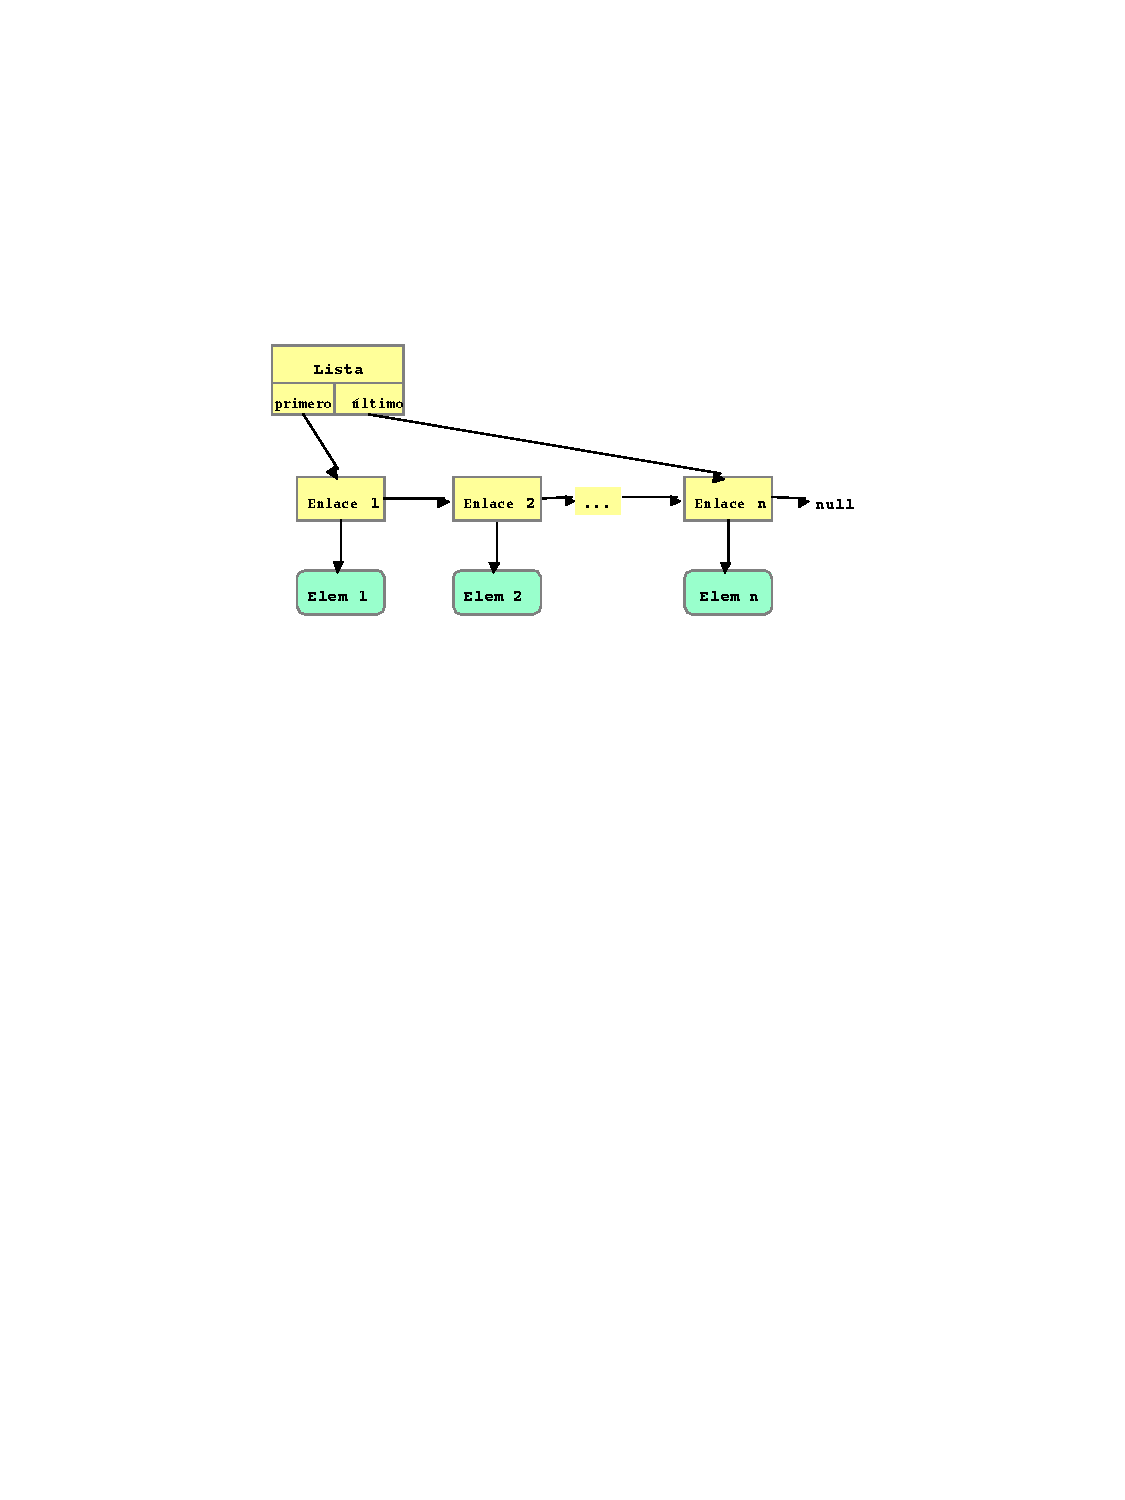
\includegraphics[width=10cm]{images/esquema.pdf}
				\end{center}
			\end{block}
		\end{frame}

        \begin{frame}
			\frametitle{Almacenamiento M\'ultiples}
			\framesubtitle{ArrayList}

			\begin{block}{Operadores}
			    {\scriptsize
			        \textcolor{blue}{-} Acceder a los elementos usando \emph{get}(i). \\ \vspace{0.25cm}
                    \hspace{1cm} \textcolor{blue}{public void} \textbf{mostrar}(ArrayList v) \{ \\
                    \hspace{1cm} \\
                    \hspace{2cm} \textcolor{blue}{for} (\textcolor{blue}{int} i = 0; i $<$ v.\emph{size}(); i++) \{ \\
                    \hspace{3cm} System.\emph{\textcolor{green}{out}}.println(v.\emph{get}(i));\\ 
                    \hspace{2cm} \} \\
                    \hspace{1cm} \} \\ \vspace{0.25cm}
			        \textcolor{blue}{-} Modificar los elementos usando \emph{set}(i).\\ \vspace{0.25cm}
                    \hspace{1cm} \textcolor{blue}{public void} \textbf{cambiar}(ArrayList v) \{ \\
                    \hspace{1cm} \\
                    \hspace{2cm} \textcolor{blue}{for} (\textcolor{blue}{int} i = 0; i $<$ v.\emph{size}(); i++) \{ \\
                    \hspace{3cm} v.\emph{set}(i, \textcolor{blue}{null});\\ 
                    \hspace{2cm} \} \\
                    \hspace{1cm} \} 
			    }
			\end{block}
		\end{frame}

\begin{frame}
			\frametitle{Almacenamiento M\'ultiples}
			\framesubtitle{Arreglos}
\begin{exampleblock}{Ejercicios}
			    {\scriptsize
				    Escriba un programa que cree un vector din\'amico que contenga  10  autos, cada auto posee como atributos: marca, modelo y valor. Se requiere recorrer el arreglo creado con autos y obtener el  promedio del valores.
			    }
			\end{exampleblock}
		\end{frame}

        \begin{frame}
			\frametitle{Almacenamiento M\'ultiples}
			\framesubtitle{Arreglos}

			\begin{exampleblock}{Ejercicios}
			    {\scriptsize
				    Escriba un programa que cree un vector din\'amico que contenga 15 objetos de tipo num\'ericos (aleatorios). Verifique el tama\~no del vector (utilizando el m\'etodo \emph{size()}) e imprima los elementos. Luego, elimine los objetos de la posici\'on 3, 7, 11 y 13. Verifique nuevamente el tama\~no del vector. Modifique los valores de la posici\'on 2 y 6 (los nuevos valores deben ser ingresados por la entrada est\'andar). Muestre los nuevos valores del vector.                    
			    }
			\end{exampleblock}
		\end{frame}


			
		\begin{frame}
			\frametitle{Preguntas}

			\hspace{4cm}\huge{Preguntas ?}
		
		\end{frame}
	\end{document}
\usetheme{default}
\usetheme{JuanLesPins}
\usetheme{Goettingen}
\usetheme{Szeged}
\usetheme{Warsaw}

\usecolortheme{crane}

\usefonttheme{serif}
\usefonttheme{structuresmallcapsserif}